\chapter*{Introduction}
\addcontentsline{toc}{chapter}{Introduction}
E-mail is an indisposable communication medium of the current Internet. Even though the concept of e-mail was developed a long time ago, it still dominates many areas of the communication, especially in commercial and governmental environments. In these days, almost every Internet user has at least one e-mail account.

There is a vast amount of software that was developed for supporting the e-mail communication: various mail exchange agents and mail servers take care of the message transfer among users' mailboxes, and various interfaces that are supposed to simplify the e-mail handling for the end-users.

This thesis concerns the end-user interfaces.
Currently, the most popular and user-friendly e-mail interfaces are those based on web technologies (accessible via browsers), and those implemented as mobile applications. These are followed by desktop, command-line and various specialized clients. The progress of their popularity throughout last years is compared in \autoref{fig:popularity}\footnote{\texttt{https://litmus.com/blog/2016-email-client-market-share-infographic}}.
\begin{figure}
\centering
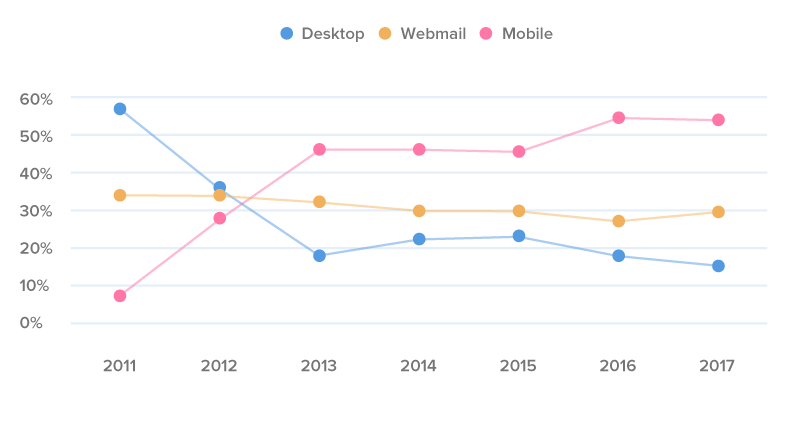
\includegraphics[width=\textwidth]{img/popularity.png}
\caption{Comparison of popularity progress of different categories of e-mail clients}
\label{fig:popularity}
\end{figure}
The popularity of the web-based and mobile clients is caused mainly by the simplicity of their deployment (no complicated configuration is usually required for their use) and the integration of many vendor-specific improvements, like search services, inter-device sharing or high availability of the service.

Despite the advantages of such interfaces, many users are forced to use less advanced solutions due to various limitations: For example, a company may choose not to submit confidential communication to its e-mail provider. Similarly, a single user may wish to process his e-mail communication locally, to avoid the issues with connectivity or provider reliability.

Such users usually deploy open-source solutions which effectively solve both the problem of vendor trust (because the software can be audited easily) and local maintainability. On the other hand, the numerous useful features (such as high-performance full-text search) and the mentioned vendor-specific improvements are typically missing in the open-source solutions.

This thesis is motivated by the concept of e-mail handling that was introduced by Google for Gmail and subsequently improved by Google Inbox. The approach completely replaces the handling of mail folders for mail organization by a more flexible use of customizable tags, and makes heavy use of Google's full-text search facilities.
Open-source solutions that would implement a decent alternative to Google Inbox are, to the best of author's knowledge, currently missing.
On the other hand, recent open-source developments have created several search engines and databases that can be used to support the underlying storage and search capabilities. Therefore, development of the alternative is possible by connecting this functionality to e-mail processing infrastructure and providing a matching modern interface for the end-user.

The goal of this thesis is to create this alternative. The specific aims include the following:
\begin{itemize}
\item high speed search for Google-like queries in large amounts of e-mails, including the tag functionality
\item integration with the e-mail processing infrastructure --- receiving, parsing, formatting and sending of e-mails
\item storing the e-mails in a reliable database
\item support for multiple users and account management
\item web-based user interface comparable to modern commercial solutions, using modern UI toolkits and frameworks to promote extensibility
\end{itemize}
The resulting open-source software package is called KamehaMail. It is possible to run KamehaMail on any modern UNIX operating system with a modern working mail server (including exim or postfix). The search functionality is provided by open-source search-engine database ElasticSearch.

This thesis is structured as follows: \Cref{mailprocess} describes the processing of e-mail messages and related Internet infrastructure. \Cref{textsearch} details the functionality of full-text search databases and their deployment in the real environments. \Cref{implementation} describes the implementation of KamehaMail, including the implementation of the backend (server part) and browser-based frontend. Performance of the resulting software is briefly benchmarked in \cref{results}. After conclusion, a short installation and user guide is provided in \cref{userguide}.

\paragraph{Related Work and Software.}
There exist a great amount of open-source web-based e-mail interfaces, such as squirrelmail, roundcube, rainloop, mailspring or notmuch-web. Most of them support full-text search using IMAP search or other own means. Yet, the handling of the e-mails as its done by Google Inbox is on whole different level on both end-user's side and the functional side. KamehaMail is trying to be as close as possible to the commercial interfaces while implementing open-source tools.
